% 双曲线的三种定义
% 极坐标系|直角坐标系|圆锥曲线|双曲线|渐近线

\pentry{圆锥曲线的极坐标方程\upref{Cone}}

\subsection{第二种定义}
我们已经知道用焦点和准线如何定义双曲线, 双曲线的极坐标方程为($e>1$)
\begin{equation}
r = \frac{p}{1 - e\cos \theta }
\end{equation}
以与极坐标系相同的原点建立直角坐标系, 要把以上方程变到直角坐标系中, 将$r = \sqrt{x^2 + y^2}$,$\cos \theta  = x/\sqrt{x^2 + y^2}$ 代入得
\begin{equation}
\sqrt{x^2 + y^2}  = p + ex
\end{equation}
两边平方且化简得
\begin{equation}
\frac{(e^2 - 1)^2}{p^2} \qty(x + \frac{ep}{e^2 - 1} )^2 - \frac{e^2 - 1}{p^2} y^2 = 1
\end{equation}
把双曲线沿 $x$ 轴正方向移动 $c$, 可得以下形式
\begin{equation}\label{Hypb3_eq4}
\frac{x^2}{a^2} - \frac{y^2}{b^2} = 1
\end{equation}
这就是双曲线的第二种定义, 从上式容易看出, 双曲线的两支是左右对称的.以上两式对比系数得
\begin{equation}
a = \frac{p}{e^2 - 1} \quad  b = \frac{p}{\sqrt{e^2 - 1} } \quad c = \frac{ep}{e^2 - 1}
\end{equation}
\begin{equation}
c^2 = a^2 + b^2
\end{equation}
用 $a, b, c$ 表示 $e,p$ 有
\begin{equation}
e = \frac{c}{a} \qquad p = \frac{b^2}{a}
\end{equation}
由离心率的定义,双曲线的焦点到准线的距离为 $p/e=b^2/c$,准线的坐标为 $c-p/e = a^2/c$.由对称性,双曲线有两个焦点和两条准线,任意一个焦点到双曲线两支的任意一点比上该点到焦点同侧准线的距离都等于离心率.

\subsection{第三种定义}
双曲线的另一种定义是, 曲线上任意一点到两个焦点距离之差等于 $2a$. 这里证明前两种定义满足该性质. 由对称性, 我们不妨只考虑右支上的某点, 令其到右焦点和右准线的距离分别为 $r_1$ 和 $d_1$, 到左焦点和左准线的距离分别为 $r_2$ 和 $d_2$. 由离心率的定义, 有
\begin{equation}
e = \frac{r_1}{d_1} = \frac{r_2}{d_2} = \frac{r_2 - r_1}{d_2 - d_1}
\end{equation}
由于两准线之间的距离恒为 $2a^2/c$, 上式变为
\begin{equation}
r_2 - r_1 = e(d_2 - d_1) = 2a
\end{equation}
证毕.

\subsection{渐近线}
\begin{figure}[ht]
\centering
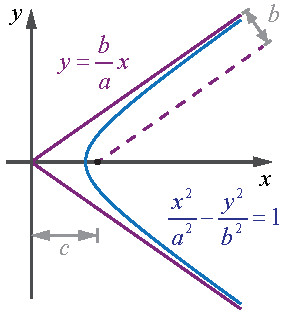
\includegraphics[width=4.8cm]{./figures/Hypb3_1.pdf}
\caption{双曲线的渐近线} \label{Hypb3_fig1}
\end{figure}

当 $x,y$ 都无穷大时, \autoref{Hypb3_eq4} 中的 $1$ 可以忽略不计,有 $y/x = \pm b/a$,渐近线与 $x$ 轴夹角为
\begin{equation}
\theta_0 = \arctan(b/a)
\end{equation}
两条渐近线到两个焦点的距离都为
\begin{equation}\label{Hypb3_eq11}
c\sin\theta_0 = c\cdot b/c = b
\end{equation}

事实上这么推导渐近线并不严谨, 在学习了高数的相关内容(见“泰勒展开\upref{Taylor}”)后, 由\autoref{Hypb3_eq4} 得
\begin{equation}
y = \frac{bx}{a} \sqrt{1-\frac{a^2}{x^2}}
\end{equation}
把根号部分关于 $a^2/x^2$ 进行泰勒展开, 有
\begin{equation}\label{Hypb3_eq13}
y = \frac ba x - \frac{ab}{2x} + \order{\frac{1}{x^3}}
\end{equation}
所以当 $x\to\infty$ 时, 就有渐进线 $y = bx/a$. 之所以要这样做, 是为了防止\autoref{Hypb3_eq13} 右边出现常数项. 如果存在常数项 $\lambda$, 那么双曲线的渐近线就是 $y = bx/a + \lambda$ 了.











